\documentclass{beamer}
\usepackage{graphicx}

\title{Learning the RNA inverse folding problem.}
\author{Carlos G. Oliver}
\date{\today}
\graphicspath{{Figures/}}



\begin{document}

\frame{\titlepage}


\frame
{
  \frametitle{Structure Prediction a.k.a. Folding}
  
  \begin{figure}
	\includegraphics[width=0.5\textwidth]{rnastruct.png}
  	\includegraphics[width=0.4\textheight]{folding.pdf} 
  \end{figure}

  
  
 \begin{itemize}
	\item  \textcolor{blue}{Input:} RNA sequence $x_1, x_2, ..., x_N$ where $x_i \in \{A, U, C, G\}$ \\
	\item  \textcolor{blue}{Output:} RNA 2D structure $\omega = \{(i, j), ... \}$ where $i$ and $j$ are indices in the sequence $x$ that are paired.
	\item Solution: Dynamic Programming + physics based rules.
	\item Current approaches achieve high accuracy in $\mathcal{O}(n^{3})$ time for sequences of length $< 200$. 
\end{itemize} 
  
  }
  
  \frame
  {
  	\frametitle{Structure Design a.k.a. Inverse Folding}
	
	
	\begin{figure}
		\includegraphics[height=0.3\textheight]{inversefold.pdf}
	\end{figure}
  
  	\begin{itemize}
		\item \textcolor{blue}{Input:} 2D Structure
		\item \textcolor{blue}{Output:} sequence whose minimum energy fold corresponds to the input.
		\item Key problem for synthetic biology and drug design.
		\item Current solutions: local search strategies
		\item \textcolor{red}{No linear time algorithms exist to solve this problem.}
	\end{itemize}
  
  }
  
  \frame{
  	\frametitle{Data}
	
	Two types of sequence-structure data:
	
	\begin{itemize}
		\item Real world
			\begin{itemize}
				\item \textcolor{red}{Rfam} databse (hand curated sequences for structural families): $\mathcal{O}(100K - 1M)$ sequences per family
			\end{itemize}
		\item Artificial
			\begin{itemize}
				\item Local search software for design: unlimited data size
			\end{itemize}
	\end{itemize}
	
}	
  \frame{
  	\frametitle{Approach: One model $\rightarrow$ one structure}
	
	
\begin{minipage}[0.2\textheight]{\textwidth}
\begin{columns}[T]
\begin{column}{0.8\textwidth}
\begin{itemize}
		\item Generate sequences belonging to one of 5 \textcolor{red}{Rfam} structural families.
		\item Given set of member sequences, generate novel likely members. 
		\item Model: RNN + LSTM 
		\item Evaluation: Covariance models, GC content, base pair distance, discriminator NN.
	\end{itemize}
\end{column}
\begin{column}{0.2\textwidth}
\includegraphics[width=2.5cm]{rnn_gen.png}
\end{column}
\end{columns}
\begin{figure}
	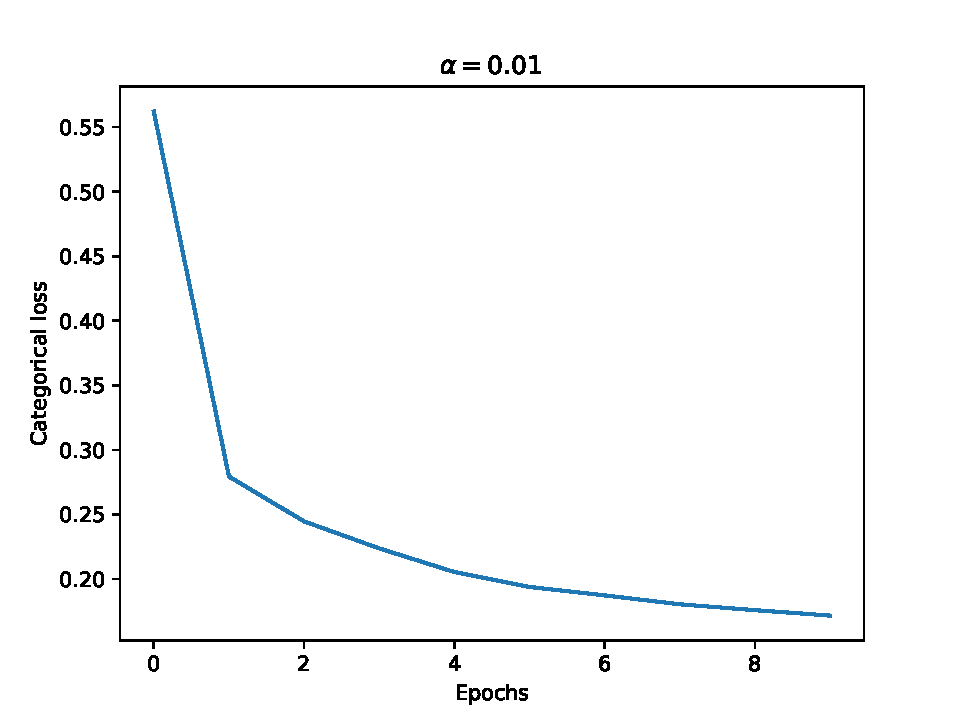
\includegraphics[height=0.4\textheight]{loss.pdf}
	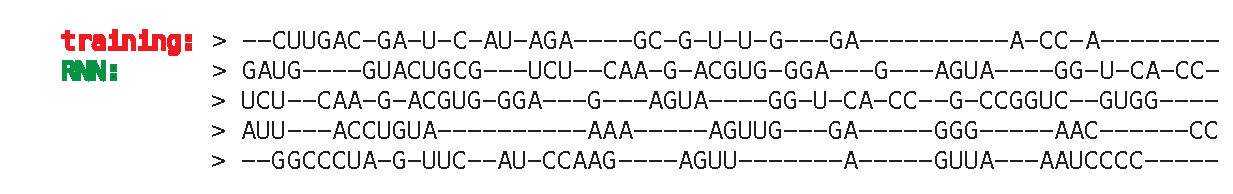
\includegraphics[width=0.5\textwidth]{genref.pdf}
\end{figure}



\end{minipage}
 }
 
 \frame{
 	\frametitle{Approach: One model $\rightarrow$ all structures}
	
	
	\begin{minipage}[0.2\textheight]{\textwidth}
\begin{columns}[T]
\begin{column}{0.8\textwidth}
\begin{itemize}
		\item Goal: generate a likely sequence for a given structure.
		\item \textcolor{blue}{Input:} vector representations $s_i \in \{0,1\}^{|\omega|}$ for each index $i$ in structure $\omega$ where 
	\end{itemize}
		
\[s_i[j] = \left\{
  \begin{array}{lr}
    1 & i  \text{  paired with  } j\\
    0 &  \text{else}
  \end{array}
\right.
\]
\end{column}
\begin{column}{0.2\textwidth}
\includegraphics[height=0.3\textheight]{rnn.png}

\end{column}
\end{columns}
\begin{itemize}
		\item \textcolor{blue}{Output:} 1 of 4 encoding of the nucleotide in $\{A, U, C, G\}$ belonging to position $i$ in structure.
		\item Approach: sequence to sequence RNN, LSTM. Recursive NN.
		\item Long term goal
	\end{itemize}


\end{minipage}		
		

 }
 

 
 
 
\end{document}
